\FloatBarrier
\subsection{Loading video data}\label{sec:load}
We process the whole night of auroral image data offline.
As described in section~\ref{sec:currentpc}, commodity computer hardware currently available allows recording all night.
On-line processing will necessarily be time-constrained, and if some unexpected event occurs (e.g. meteor, vehicle reentry) the possibly unique data would be lost as the discrimination algorithm is not tuned for such an event.

For reduced processing time, one can choose to sample every N\textsuperscript{th} frame set.
Deciding which interval to sample at is driven by the need to sample the entire night's data and extract interesting frames before it's time to record again for the next night.
Although DAW events evolve on sub-second time scales, there are generally several DAW sub-events happening in parallel and serially over 5..\unit[15]{s} intervals, with several such groups of events occurring within 1..\unit[5]{min.}
The bounds on discrimination algorithm data loading cadence $T_L$ in seconds is thus bounded by
\begin{equation}\label{eq:loadint}
T_0 < T_L < T_1.
\end{equation}
Empirically, an Intel i7 Ivy Bridge CPU yields $N \gtrsim 20$ and with camera kinetic rate $T_K=\unit[20]{ms}$, $T_0 \sim \unit[400]{ms}$.
Given typical event duration $\unit[5]{s} \lesssim T_E \lesssim \unit[15]{s}$, $T_1 \sim \unit[2]{s}$.
Thus \eqref{eq:loadint} becomes
\begin{equation}\label{eq:actload}
0.4 < T_L < 2.
\end{equation}
As computer hardware capability increases with future CPU generations, $T_0$ becomes smaller and/or more advanced discrimination algorithms may be employed.

The images are stored in a raw binary stream containing a fixed-length footer containing a sequence number and other user-chosen per-frame metadata.
DMC and HiST phase 1 used a four byte footer for this purpose.
For simplicity, the experiment configuration is stored in a standard XML file.
The raw binary file will be more than \unit[1]{TB} in size for a whole night recording, so for ease of download and user experience auroral events of interest are repacked into an losslessly compressed HDF5 format file.
The HDF5 file is chunked, one image per chunk for fastest reading, combined with metadata like the format used by the Madrigal geospace data repository \citep{madrigal} and uploaded to Zenodo.

Auroral image histograms are not adequate to discriminate on alone since they do not contain sufficient information about the morphology. 
The ground-observed brightness of aurora is highly dependent upon viewing angle and the arrangement of the aurora along a particular viewing angle as described by~\eqref{eq:bint}.
An example auroral histogram on a clear viewing night with a few bright stars and a discrete arc away from magnetic zenith is shown in Figure~\ref{fig:diffimhist}.
\begin{figure}\centering
    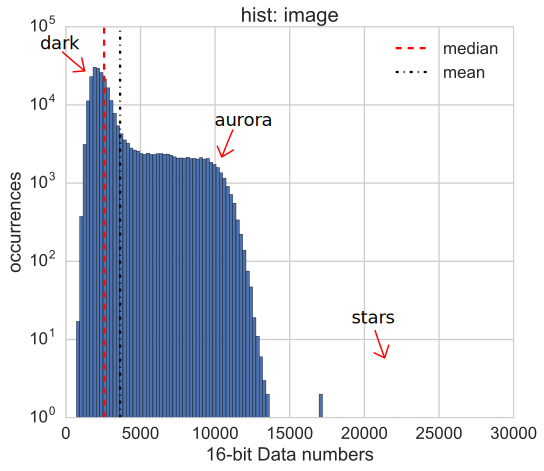
\includegraphics[width=0.7\linewidth]{gfx/diffuse-imhist}
    \caption{Histogram of discrete arc away from magnetic zenith.}\label{fig:diffimhist}
\end{figure}
Due to photon-stared low auroral video SNR, there is no clear separation between auroral intensity values and background noise, thus even adaptive intensity threshold algorithms fail.